\chapter{Methods}\label{methods}

\epigraph{The universe must be full of voices, calling from star to star in a myriad tongues. One day we shall join that cosmic conversation}{Arthur C. Clarke}

In order to simulate the evolution of hierarchical triple-star systems with a  Roche-lobe-filling outer star, various physical processes, such as stellar evolution, gravitational dynamics, and hydrodynamics needs to be considered. First, I employ the stellar evolution code MESA \citep{paxton2010modules,paxton2013modules,paxton2015modules,paxton2019modules} to model the evolution of the system's stars prior to outer stars' \ac{rlof}. Once the outer star reaches the stage where it approximately fills its Roche lobe, I pause the stellar evolution simulation and convert the one-dimensional stellar structure into a three-dimensional hydrodynamical model. This 3D hydrodynamical model of the outer star is then relaxed, using GADGET-2 \citep{springel2005cosmological}, and placed in orbit around the binary star. The inner binary components are seen as point masses and their gravitational dynamics are handled by Huayno \citep{pelupessy2012n}. Subsequently, I monitor the intricate hydrodynamics of the mass transfer from the Roche lobe-filling outer star to the inner binary for multiple orbits, while simultaneously keeping track of the three stars gravitational dynamics and the outer star gas hydrodynamics. 

In this chapter I present in detail all the aforementioned steps. In each step I discuss the exploration of different parameters, the underlying assumptions of the models and their physical justification.

\section{Stellar evolution}\label{sec:stellar_evolution}

The stellar evolution calculations in this work are performed using the normal AMUSE parameters for MESA, with solar metallicity as the input.
MESA allows me to track the independent evolution of the triple system components and obtain estimations of their properties at the beginning of RLOF. In this work, I allow the tertiary to evolve until $R_{stop} = 1.1 \times R_{L}$, see \cref{eq:roche_lobe}. The consequence of this choice will be discussed in detail in \cref{simulations}.

By the time the outer star approaches the radius of its Roche lobe, all three stars have lost some mass, while the tertiary's radius is much bigger than when it was formed. In order to accurately evaluate the Roche lobe sizes,  I need to estimate the masses of the stars at the RLOF moment. Unfortunately, $\xi$ Tau's age is not known, but mass-loss via winds during the main sequence is expected to be unimportant for low- and intermediate- mass stars, see \cref{sub:winds}.

Despite that, I track the evolution of the tertiary's mass and radius profile. As expected, radiation-driven mass-loss proved negligible in this mass regime. For cold winds, I utilize Reimer's, see Eq. \eqref{eq:reimer}, and Blocker's, see Eq. \eqref{eq:blocker}, mass-loss prescriptions using commonly used scaling factors of $\eta = 0.5$ and $\eta = 0.1$, respectivelly. 
\begin{figure}[H]
    \centering
    \begin{subfigure}{.5\textwidth}
    \centering
    \includegraphics[width=0.9\textwidth]{Thesis/graphs/giant_1-1mass_loss.pdf}
    \label{fig:mass_loss}
    \end{subfigure}%
    \begin{subfigure}{.5\textwidth}
    \centering
    \includegraphics[width=0.9\textwidth]{Thesis/graphs/giant_1-1radius.pdf}
    \label{fig:radius_profile}
    \end{subfigure}
    \caption{ Mass and radius evolution of a 5.5 M$_{\odot}$ star at solar metallicity until RLOF. ZAMS and TAMS are noted by black circles, while the start and end of helium burning by black squares. I create the stellar evolution models using MESA \citep{paxton2010modules,paxton2013modules,paxton2015modules,paxton2019modules}.}
\end{figure}
The tertiary loses less than $1\%$ of its 
initial mass, while the expected mass-loss from the binary components is even smaller, because less massive, and thus less luminus, stars will have weaker winds. As a result, I do not correct for mass-loss and use the parameters listed in  \cref{tab:system_orbit_param}.  

At this point, I also assume that the mass lost through winds has no effect on the stars. This assumption would be false in the case of more massive stars. As mass escapes from the star's surface, it carries angular momentum and can change the inner and outer orbital parameters. Furthermore, some of the escaped mass can be accreted, complicating the evolution of the two orbits even further. Given the small amount of mass loss, the aforementioned assumption is safe in this case.

In \cref{fig:HR_ROLF}, I present the evolution of the tertiary on the HR diagram until the moment of RLOF and in \cref{tab:tertiary_param_ROLF} I summarize the tertiary's important stellar parameters. 
\begin{figure}[H]
    \centering
    \includegraphics[width=0.9\textwidth]{Thesis/graphs/HR_1-1ROLF.pdf}
    \caption{Evolution of 5.5 M$_{\odot}$ at solar metallicity until the moment of RLOF. ZAMS and TAMS are noted by black circles, while the start and end of helium burning by black squares. The evolutionary phases have categorized in different colors similar to \cref{fig:HR_evolution}. I calculate the track using MESA \citep{paxton2010modules,paxton2013modules,paxton2015modules,paxton2019modules}. The dashed lines show lines of constant radii by means of the Stefan–Boltzmann law.}
    \label{fig:HR_ROLF}
\end{figure}
\begin{table}[H]
    \centering
    \begin{tabular}{| c | c |}
       Parameter & Value \\
       \hline 
       M$_{RLOF}$ & 5.5 (M$_{\odot}$) \\
       R$_{RLOF}$ & 91.36 (R$_{\odot}$) \\
       L$_{RLOF}$ & 2262 (L$_{\odot}$) \\
       t$_{RLOF}$ & 82.36 (Myr) 
    \end{tabular}
    \caption{ $\xi$ Tau parameters at the beginning of RLOF. From top to bottom the tertiary's mass, radius, luminosity and age.}
    \label{tab:tertiary_param_ROLF}
\end{table}
The tertiary is expected to overflow its Roche lobe during the early AGB phase, after helium exhaustion, leading to a type C mass transfer. Hence, I expect that the envelope will be convective, see \cref{sec:single_star_evolution}.

In order to verify that, I present a Kippenhahn diagram of the tertiary, see \cref{fig:kippen_plot}. This diagram displays the structural evolution of the star from the core to the photosphere. The vertical axis represents the position within the star in terms of enclosed mass and the horizontal axis represents the number of the models, which are translated to stellar age (hence the x-axis is not linear). In this diagram, one can see how different regions are discerned: The white parts are the radiative regions, the stripped parts represent the convective regions, and the variation of the color represent the intensity of the energy generation at various regions in arbitrary units. Darker color indicate that more energy is produced.
\begin{figure}[H]
    \centering
    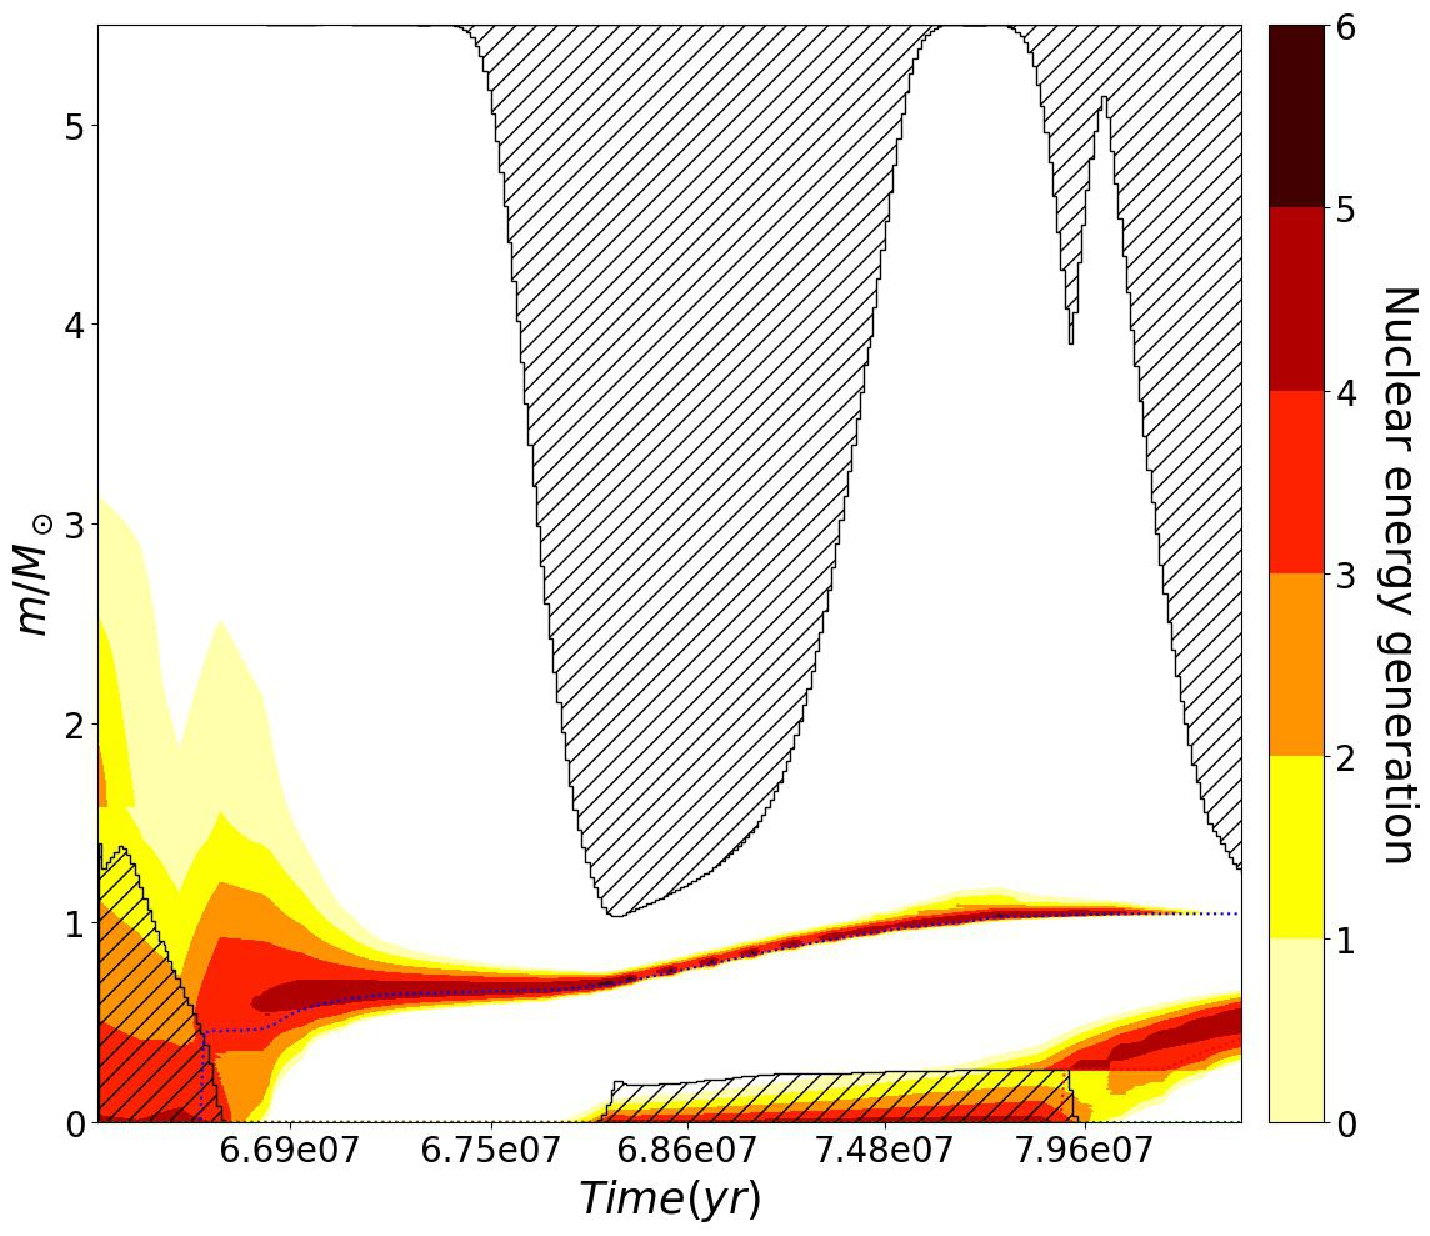
\includegraphics[width=0.9\textwidth]{Thesis/graphs/Kippen_ROLF_Schw.pdf}
    \caption{Kippenhahn diagram of $\xi$ Tau outer component until the onset of RLOF using Schwarzwild criterion, see Eq. \eqref{eq:Schwarzwild_criterion}. The vertical axis represents the position within the star in terms of enclosed mass and the horizontal axis represents the number of the models which are translated to stellar age. The white parts are radiative regions, the stripped parts represent convective regions, and the variation of the color represent the intensity of the energy generation at various regions in arbitrary units. Darker color indicate that more energy is produced. I create the graph using MESA \citep{paxton2010modules,paxton2013modules,paxton2015modules,paxton2019modules}.}
    \label{fig:kippen_plot}
\end{figure}
At the moment of RLOF, the convective envelope has penetrated deep inside the star close to the actual core. Hence, in this case, convection defines the mechanical structure of the envelope. This is critical for the 3D hydrodynamical model and it is discussed in detail in \cref{sec:1D_to_3D}. 

Given the parameters in \cref{tab:tertiary_param_ROLF}, I also calculate the relevant characteristic timescales of the tertiary, see \cref{sec:timescales}, which are listed in \cref{tab:tertiary_timescale_ROLF}.
\begin{table}[H]
    \centering
    \begin{tabular}{| c | c |}
       Timescale & Duration \\
       \hline
       $t_{dyn}$ & 4.85 day\\
       $t_{th}$ & 4585.78 yr 
    \end{tabular}
    \caption{ Tertiary timescales at the beginning of RLOF.}
    \label{tab:tertiary_timescale_ROLF}
\end{table}
\begin{comment}
In \cref{tab:system_orbit_param_ROLF} I summarize the important parameters of the system at the moment of RLOF. 
\begin{table}[H]
    \begin{adjustbox}{width=1\textwidth}
    \small
    \centering
    \begin{tabular}{| c c c c c c c c c c|}
       M$_1$ (M$_{\odot}$) & 
       M$_2$ (M$_{\odot}$) &
       M$_3$ (M$_{\odot}$) & $\alpha_{in}$ (au) &
       $\alpha_{out}$ (au) &
       $\epsilon_{in}$ &
       $\epsilon_{out}$ &
       $R_{RLOF}$ (au) &
       $t_{RLOF}$ (Myr) &
       $M_{RLOF}$  (M$_{\odot}$) \\
       \hline
       3.2 & 3.1 & 5.5 & 0.133 & 1.24 & 0.0 & 0.15 & 0.423 & 82.36 & 5.5
    \end{tabular}
    \end{adjustbox}
    \caption{ Orbital parameters of $\xi$ Tau system at the beginning of RLOF}
    \label{tab:system_orbit_param_ROLF}
\end{table}
Given these parameters, I also calculate the relevant characteristic timescales of the tertiary, which are listed in \cref{tab:tertiary_timescale_ROLF}.
\begin{table}[H]
    \centering
    \begin{tabular}{| c | c |}
       Timescale & Duration \\
       \hline
       $t_{dyn}$ & 4.85 day\\
       $t_{th}$ & 4585.78 yr 
    \end{tabular}
    \caption{ Tertiary timescales at the beginning of RLOF.}
    \label{tab:tertiary_timescale_ROLF}
\end{table}
\end{comment}
Note that the default parameters of MESA withing AMUSE do not include overshooting. However, I perform one test taking into account overshooting with $f=0.016$ \citep{herwig2000evolution}. On one hand, the MS lifetime extends, RLOF occurs $~10Myr$ later in the evolution, while the stellar core is more massive. On the other hand, the impact on the structure of the envelope's outer layers at the moment of RLOF is negligible. This is the region of highest interest for my mass transfer simulations, thus I proceed with models without overshooting. Nevertheless, it is worth mentioning that for $f=0.016$, RLOF occurs before helium exhaustion leading to a type B mass transfer.

\section{Converting the 1D stellar evolution model to a 3D gas particle distribution}\label{sec:1D_to_3D}

In addition to fundamental parameters such as mass, radius, etc., MESA enables to access the stars internal structure. This information is essential to convert the 1D stellar models into 3D hydrodynamical realizations, providing a more comprehensive understanding of the physical processes involved in \ac{rlof} and the resulting mass transfer in these systems.

When the radius of the outer star exceeds its Roche limit, the 1D stellar evolution model is converted to a collection of \ac{sph} particles. This is accomplished by requesting the radial stellar structure profiles for density, temperature, mean molecular weight, and radius from the stellar evolution code. MESA divides a star into a series of spherical shells, which are represented by arrays in which these parameters are recorded. Following that, I produce a kinematically cold set of $N$ particles of mass $M_{RLOF}/N$ in a uniform spherical distribution. I now scale the particle locations radially to fit the density profile from the star up to its outer radius.

\subsection{Stellar Interior}\label{sub:core}

Because of the usage of equal-mass particles and the high concentration of stellar cores, the majority of the particles, and therefore the maximum resolution, will be in the stellar core, whereas the star's outer edge will be barely resolved. However, I want to investigate the hydrodynamical factors that dominate the star's outer layers in order to gain meaningful insights into the mass transfer process. To achieve that, I replace the stellar core with a single mass point, because the interior of the Roche lobe filling star barely affects the dynamics of the outer layers on the short-dynamical timescales associated with \ac{rlof} \citep{deupree2005structure}. This technique not only provides higher resolution of the outer layers but also helps to circumvent computational run time constraints by using less particles. This procedure is coded in the standard AMUSE routine called $star\_to\_sph.py$.
\begin{figure}[H]
    \centering
    \includegraphics[width=0.9\textwidth]{Thesis/graphs/ROLF_density_profile.pdf}
    \caption{Radial density profile of the  $\xi$ Tau outer component at the onset of \ac{rlof} (blue line). MESA's 1D density profile of the tertiary is shown by the solid blue line. The shaded region represents 99.9\% of the star's enclosed mass. The dotted lines depict \ac{sph} models with varied core masses, M$_{core}$, which correspond to fractions of 0.1, 0.255, 0.5, and 0.75 of the overall mass of 5.5 M$_{\odot}$, while the larger points correspond to core particle densities, respectively.}
    \label{fig:stellar_density_ROLF}
\end{figure}
The core particle's mass is unrelated to the mass of the hydrogen-exhausted stellar core, but rather a solution to the computational challenges of modeling big stars without changing the stellar envelope's behavior. Furthermore, it as a pure gravitational point mass with no pressure or internal energy. I investigate core masses corresponding to different percentages of the star's mass at the onset of \ac{rlof}, which are listed in \cref{tab:core_masses_ROLF}. 
\begin{table}[H]
    \centering
    \begin{tabular}{| c |}
       M$_{core}$  \\
       \hline
       10\% M$_{RLOF}$\\
       25\% M$_{RLOF}$\\
       50\% M$_{RLOF}$\\
       75\% M$_{RLOF}$
    \end{tabular}
    \caption{ Different core masses for the 3D hydrodynamical model of the tertiary at the beginning of \ac{rlof}}
    \label{tab:core_masses_ROLF}
\end{table}
Lower core masses, M$_{core}$ $\leq$ 0.2M$_{RLOF}$, retain the problematic high density in the core, but larger core masses, M$_{core}$ $\geq$ 0.4 M$_{RLOF}$, cause the density in the envelope to depart significantly from the stellar structure model. This trend is apparent in \cref{fig:stellar_density_ROLF}. I adopt M$_{core}$ = 0.255 M$_{RLOF}$ (= 1.4 M$_{\odot}$), which successfully overcomes the problematic high density inner stellar region and is in good agreement with envelopes' density profile.

After investigating different number of particles, $N$, I adopt $N=50000$  due to the fact that higher $N$ numbers does not offer a significant improvement in resolving the outer layers of the star, while increase significantly the computational run time of the simulations.  Hence, each particle represents $M_{RLOF}/N = 11 \times 10^{-4}$ M$_{\odot}$ of gas.

\subsection{Stellar envelope: Convective case}\label{sub:envelope_conv}

Following the distribution of particles based on the 1D density profile of the tertiary, I need to accurately specify important thermodynamic properties of the envelope (3D model), such as specific internal energy and specific entropy. Because the pressure of a gas is related to its internal energy, I need to examine the pressure sources in the envelope. In general, the pressure in a non-degenerate stellar interior will be given as 
\begin{equation}\label{eq:pressure}
    P(r) = \frac{1}{3} \alpha T(r)^4+ \frac{\mathcal{R}}{\mu(r)} \rho(r) T(r)
\end{equation}
where $\alpha$ and $\mathcal{R}$ are the radiation and universal gas constants, respectively. The first term in \cref{eq:pressure} is the radiation pressure exerted by photons and it will be dominant for massive hot stars, while it can be neglected for cool stars \citep{pols2011stellar}.

Although, I do not expect the radiative component to be dominant in a $5.5$ M$_{\odot}$ star, I verify this assumption. In \cref{fig:eos}, I present, in black dashed lines, the boundaries between different sources of pressure. The coloured regions mark what pressure source dominate the equation of state in the considered regime of temperature and density, namely the radiation, the ideal gas or the (non-relativistic / relativistic) electron degeneracy pressure. The blue line corresponds to the internal structure of the tertiary at moment of \ac{rlof}. Starting from right to left, I follow the density and temperature of the star from the core to its surface. The black $x$ indicate, for decreasing $\rho$, the part of the star containing 1.375 M$_{\odot}$, 2.75 M$_{\odot}$, 4.125M$_{\odot}$ and 5.5 M$_{\odot}$, respectively. These values correspond to 25\%, 50\%, 75\% and 100\% of the star's enclosed mass.
\begin{figure}[H]
    \centering
    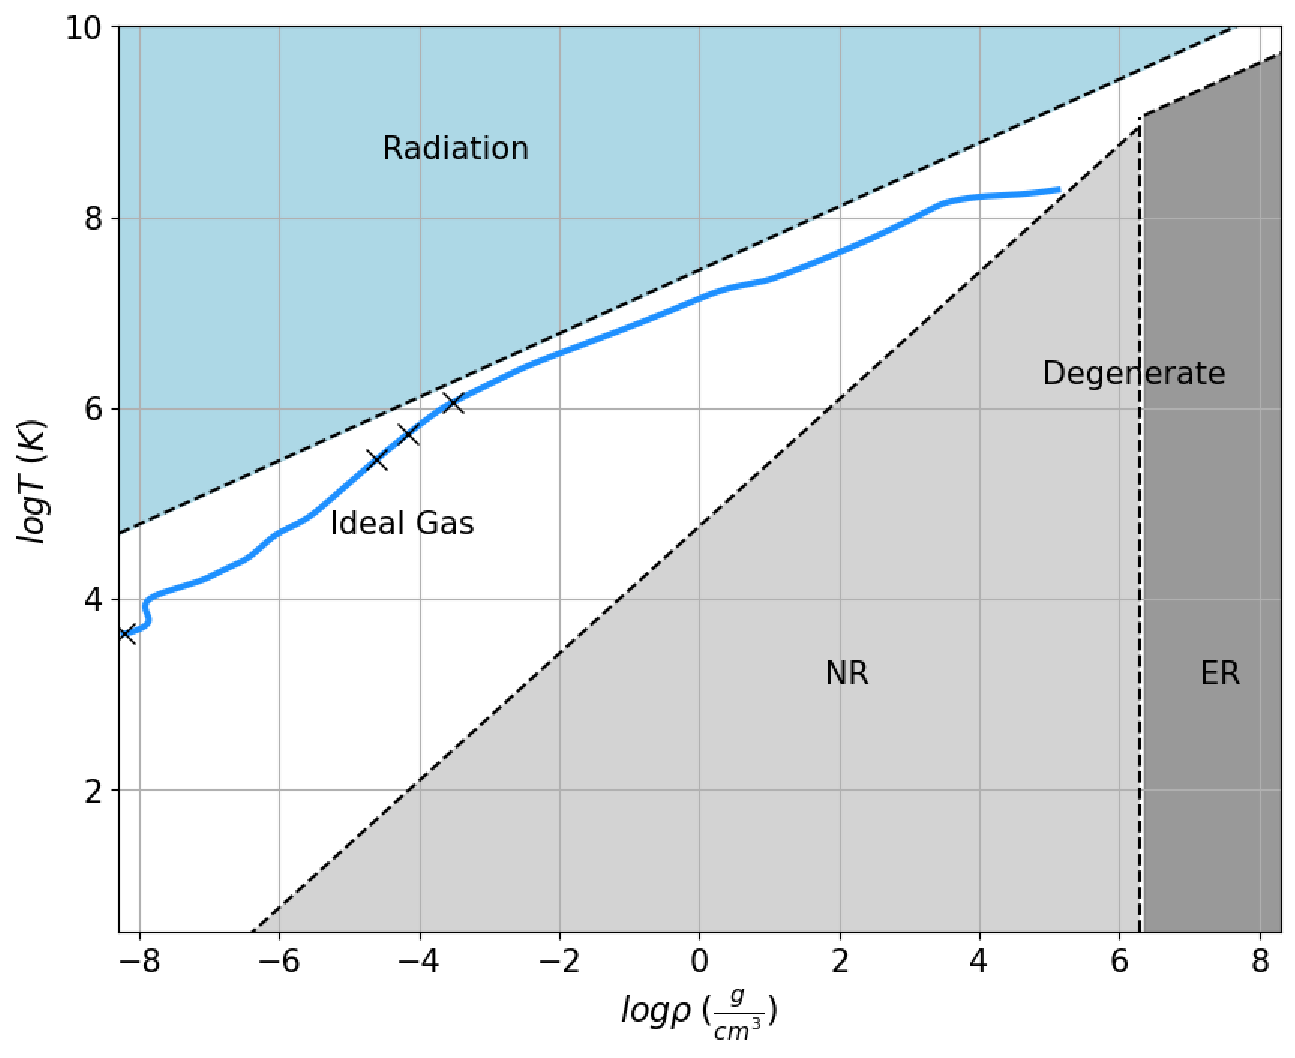
\includegraphics[width=0.9\textwidth]{Thesis/graphs/eos.pdf}
    \caption{ The radial structure of the outer star at the moment of \ac{rlof} in the  temperature-density plane. I calculate the stellar profile using MESA \citep{paxton2010modules,paxton2013modules,paxton2015modules,paxton2019modules}.}
    \label{fig:eos}
\end{figure}
At the moment of \ac{rlof} the pressure within the envelope is dominated by the ideal gas component, see \cref{fig:eos}. Thus I can indeed neglect the radiative part of \cref{eq:pressure}. Using
\begin{equation}\label{eq:pressure_ideal_gass}
    P(r) =  \frac{\mathcal{R}}{\mu(r)} \rho(r) T(r)
\end{equation}
each particle is allocated a unique specific internal energy based on the temperature and mean molecular mass profiles:
\begin{equation}\label{eq:internal_energy}
    u(r) = \frac{3}{2} \frac{k_B T(r)}{\mu(r)},
\end{equation}
where $k_B$ is the Stefan-Boltzmann constant, $T(r)$ and $\mu(r)$ the temperature and mean molecular mass profiles, respectively.

The particles at this point are kinematically cold meaning that their specific kinetic energies are zero and only their internal and potential energies contribute to the total energy of the gas. This is illustrated in \cref{fig:kinetic_internal_energies}, where I present 2D maps of the kinetic and internal particle energies, respectively.
\begin{figure}[H]
    \centering
    \begin{subfigure}{.5\textwidth}
    \centering
    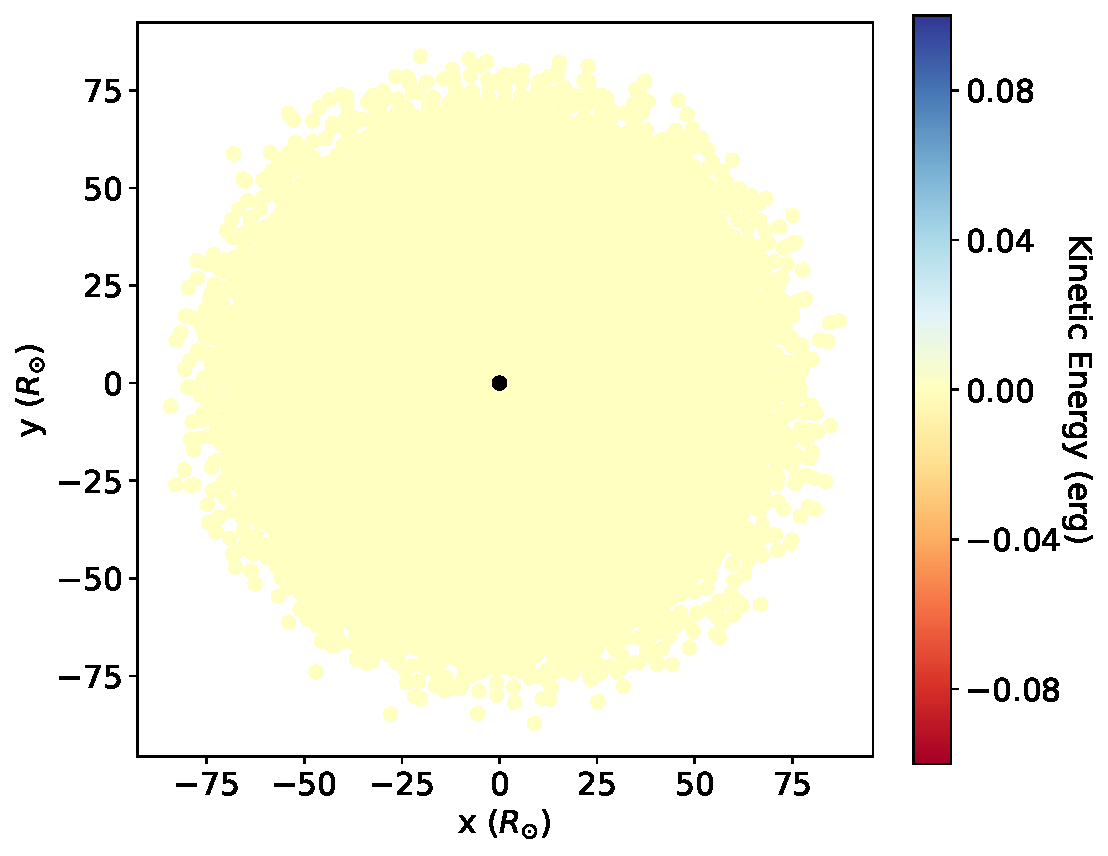
\includegraphics[width=0.9\textwidth]{Thesis/graphs/tertiary_kin_energy_before_relaxation.pdf}
    \label{fig:mass_loss}
    \end{subfigure}%
    \begin{subfigure}{.5\textwidth}
    \centering
    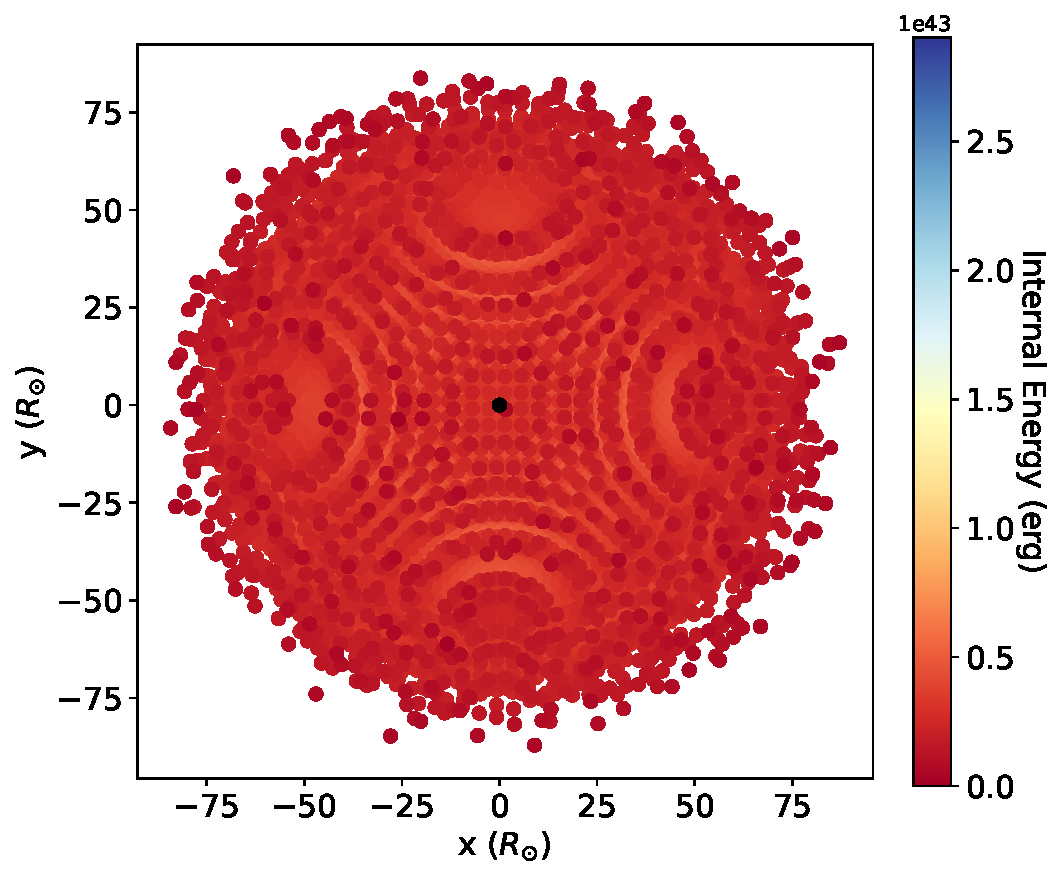
\includegraphics[width=0.9\textwidth]{Thesis/graphs/tertiary_internal_energy_before_relaxation.pdf}
    \label{fig:radius_profile}
    \end{subfigure}
    \caption{ Kinetic and internal energies of the gas particles after converting the 1D stellar evolution model to a 3D gas particle distribution. The black point corresponds to the core particle which is a pure gravitational point mass with no pressure or internal energy.}
    \label{fig:kinetic_internal_energies}
\end{figure}
Another important parameter of the gas is its specific entropy. It is often mathematically simpler, although not formally necessary, to define an entropic variable $A$. The entropic variable $A$ is closely linked (but not identical) to the specific entropy and it is defined as
\begin{equation}\label{eq:entropic_variable}
    A(r) \equiv \frac{P(r)}{\rho(r)^{\gamma_{ad}}}
\end{equation}
where $\gamma_{ad}$ is the adiabatic index, and $P(r)$ and $\rho(r)$ the pressure and density profiles, respectively. 

The evaluation of the original entropic profile $A(r)$ of the stellar envelope is not trivial and one needs to consider the relevant pressure sources, see \cref{eq:pressure}. In a radiation-dominated gas, $\gamma_{ad} = 4/3$ is a more suitable adiabatic index (this is in general true when extremely relativistic particles dominate), while for a mixture of gas and radiation, $4/3 \leq \gamma \leq 5/3$. However, at the moment of \ac{rlof}, see \cref{fig:eos}, ideal gas is the dominant radiation pressure source, thus considering \cref{eq:internal_energy} and \cref{eq:entropic_variable}, I calculate the entropic profile $A(r)$ with $\gamma = 5/3$, such as:
\begin{equation}\label{eq:entropic_variable_2}
    A(r) = \frac{2}{3} u(r) \rho(r)^{-2/3}.
\end{equation}

\subsection{Stellar envelope: Radiative case}\label{sub:envelope_rad}

In the previous subsections I showed how I model $\xi$ Tau's outer component. The presented method works pretty well due to the fact that the envelope is convective at the onset of \ac{rlof}. I tested the scenario of \ac{rlof} occurring at different phases of the evolution, when the envelope is radiative, and for different initial stellar masses. Hence, I present the additional parameters that need to be considered in the case of a radiative envelope. These key points can be incredibly valuable and time-saving for future work using the same method.

Low-mass, thus cold, stars have convective envelopes during their evolution, while massive stars with M$>16$M$_{\odot}$ remain with a radiative envelope pretty much until the end of their lives. Intermediate- and high-mass stars' envelopes (M  $<16$M$_{\odot}$) can be either convective or radiative depending on the evolutionary phase in which \ac{rlof} occurs, see \cref{sec:single_star_evolution}. 
\begin{figure}[H]
    \centering
    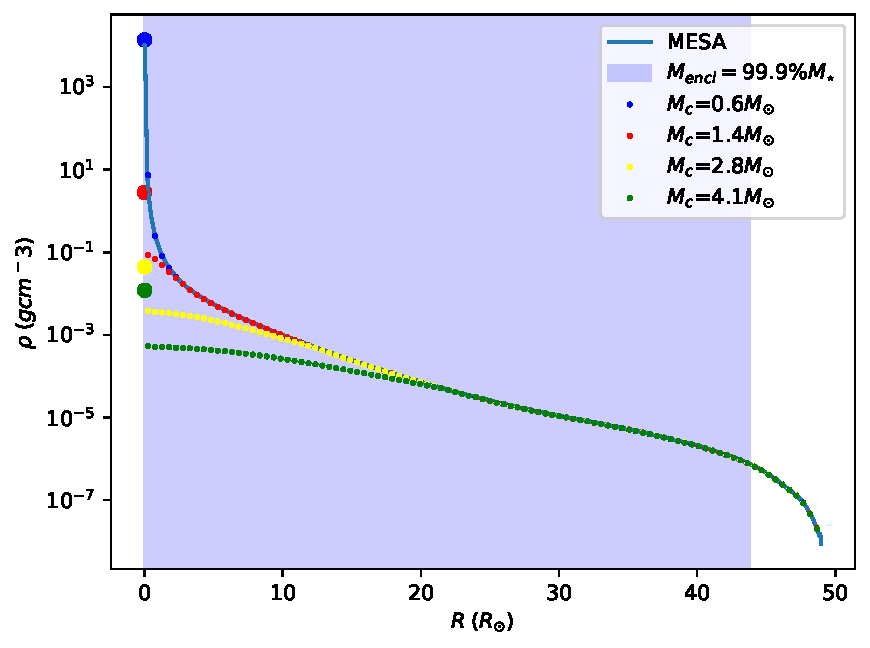
\includegraphics[width=0.9\textwidth]{Thesis/graphs/density_profile_radiative_envelope.pdf}
    \caption{Radial density profile of the  $\xi$ Tau outer component at $t=78.3$ Myr (blue line), when the star is in its helium-burning phase and has a fully radiative envelope. MESA's 1D density profile of the tertiary is shown by the solid blue line. The shaded region represents 99.9\% of the star's enclosed mass. The dotted lines depict \ac{sph} models with varied core masses, M$_{core}$, which correspond to fractions of 0.1, 0.255, 0.5, and 0.75 of the overall mass of 5.5 M$_{\odot}$, while the larger points correspond to core particle densities, respectively.}
    \label{fig:density_profile_radiative}
\end{figure}
The density within a convective envelope falls of with pressure $\rho \propto P^{1/\gamma_{ad}}$, see \cref{eq:adiabatic_eos}. If the envelope is stable against convection, the density gradient must vary more steeply with pressure than for an adiabatic change by definition. This means that radiative envelopes are less dense in the outer layers and more centrally concentrated than convective envelopes \cite{pols2011stellar}. This is reflected in \cref{fig:density_profile_radiative}, where I plot the tertiary's radial density profile at $t=78.3$ Myr, when the star is in its helium-burning phase and has a fully radiative envelope, see \cref{fig:kippen_plot}.

Modeling the radiative envelope case is more challenging. From the computational point of view, the problem branches in to two sub-problems. First, a comparison between \cref{fig:stellar_density_ROLF} and \cref{{fig:density_profile_radiative}} immediately reveals the difference in scales. More specifically, in the radiative case someone needs to resolve 6-8 orders of magnitude in density. In \cref{fig:density_profile_radiative}, I use $N=10^6$ particles and still the outer layers of the star are not very well resolved. This is a direct consequence of the density's profile high steepness and the use of equal mass particles. In general, the use of equal mass particles provides good resolution in high-density regions, however, only poorly resolves low-density regions. Second, using $N$ of 6 orders of magnitude, will result in extremely long computational time, as the CPU simulation time is not linear function of $N$, but rather the CPU time increases with the number of \ac{sph} particles as $NlogN$.

The problematic steepness of the density profile becomes more severe for high-mass stars. Additionally, as stellar mass grows so does the importance of radiation pressure. From a physics standpoint, someone must estimate the importance of radiation in order to accurately define the thermodynamic properties of the gas using \cref{eq:pressure}, \cref{eq:entropic_variable} and a proper adiabatic index, $\gamma_{ad}$.

In conclusion, the method is preferable for modeling low- and intermediate-mass stars with convective envelopes. For high-mass stars, even if the thermodynamic properties of the gas are defined properly, the intrinsic steepness of the density profile will remain.  Hence, a very high number of \ac{sph} particles are needed to resolve the stellar envelope, which result in very long computational times. 




\begin{comment}
    This parameter will be important in order to adjust correctly thermodynamic properties of the gas inside the softened zone.
\end{comment}

\section{Bringing the 3D hydrodynamical model in hydrostatic equilibrium}

Up to this point, I have specified most of the 3D hydrodynamical model's parameters, which would be simulation's starting point. However, an extremely unstable model would result from entering these values into GADGET-2, where the gas particles would quickly reach arbitrary high velocities and escape.

There are two causes for this behavior, and as a result, there are two additional phases I must complete before I can produce a smooth and stable 3D hydrodynamical model. The first is related to the softening length of the core particle, while the second is related to the initial gas particle accelerations as being calculated by GADGET-2 via gravitational forces and pressure gradients. In the next two subsection I will expand upon how I tackle these challenges. 

Furthermore, I consider an adiabatic \ac{eos}, see \cref{eq:adiabatic_eos}, with $\gamma_{ad} = 5/3$, in GADGET-2 for the gas. Hence, the simulaitons include adiabatic cooling and heating due to expansion and contraction of the gas, respectively. This decision is predicated on the fact that the simulation run time is more than two orders of magnitude shorter than the $t_{th}$ of the tertiary, see \cref{tab:tertiary_timescale_ROLF}. If $t_{th}$ was significantly shorter than the current value, an isothermal \ac{eos} may be a better choice. In order to test this assumption, I run one simulation using an isothermal \ac{eos}. As expected, the model proved extremely unstable with the envelope escaping freely since it is not affected by adiabatic cooling.

\subsection{Core particle softening length}

Since I consider the core particle to be a pure gravitational point mass with no pressure or internal energy, I need to avoid the star from collapsing on itself.
To achieve that, I use Plummer softening, $\epsilon$, to soften the core particle. Similar with GADGET-2, I adopt the conventional cubic spline of \cite{monaghan1985refined}, which drops to zero smoothly at $2.8 \epsilon$, see Eq. \eqref{eq:spline_kernel}. The density and internal energy inside the softened zone are adjusted so that pressure equilibrium is maintained while the original entropic variable $A$ is preserved, see \cref{sub:envelope_conv}. 

The motivation behind that is known as entropy sorting and it is derived by simulations of stellar collisions \citep{lombardi1995collisions,lombardi2003modelling,lombardi2006stellar,gaburov2008mixing,gaburov2010onset}, where both the entropic variable and the specific entropy are preserved in the absence of shocks and increase in their presence. To put it simply, the fluid with the highest entropy should be on top of the fluid with the lowest entropy in order to establish hydrodynamic stability. 

Defining a good $\epsilon$ has been proved a major challenge. I run a series of short convergence tests varying the number of particles $N$ and the core particle mass, $M_c$. The tests proved that the choice of the softening length, $\epsilon$, depends weakly on $N$, and strongly on $M_c$, which is related to the tertiary's mass at the moment of \ac{rlof}, see \cref{tab:core_masses_ROLF}. I demand two criteria to be fulfilled, at the same time, for selecting a good softening length:
\begin{itemize}
    \item The selected $M_c$, and hence the respective softening length, should result to a 3D density profile which agrees with MESA's 1D density profile.
    \item For a given $M_c$, and hence the respective softening length, the star should not collapse on itself at the beginning of the simulation.
\end{itemize}
The first criterion allowed me constraint my parameters' search, see \cref{fig:stellar_density_ROLF}. For the adopted $M_c$=0.255 M$_{ROLF}$, I present the parameters of the convergence tests
\begin{table}[H]
    \centering
    \begin{tabular}{| c | c | c |}
       M$_{core}$  & N & $\epsilon$/$R_{RLOF}$ \\
       \hline
       25.5\% M$_{RLOF}$ & $10^4$ & 0.1\\
       25.5\% M$_{RLOF}$ & $10^4$ & 0.15\\
       25.5\% M$_{RLOF}$ & $10^4$ & 0.2\\
       25.5\% M$_{RLOF}$ & $10^4$ & 0.25\\
       25.5\% M$_{RLOF}$ & $10^4$ & 0.3\\
       25.5\% M$_{RLOF}$ & $10^4$ & 0.4\\
       \hline
       25.5\% M$_{RLOF}$ & $50^4$ & 0.1\\
       25.5\% M$_{RLOF}$ & $50^4$ & 0.15\\
       25.5\% M$_{RLOF}$ & $50^4$ & 0.2\\
       25.5\% M$_{RLOF}$ & $50^4$ & 0.25\\
       25.5\% M$_{RLOF}$ & $50^4$ & 0.3\\
       25.5\% M$_{RLOF}$ & $50^4$ & 0.4\\
    \end{tabular}
    \caption{ Parameters of the convergence tests to adopt a softening length, $\epsilon$, for the tertiary at the beginning of \ac{rlof}.}
\label{tab:smoothing_length_exploration}
\end{table}
The tests proved that an $\epsilon \in [0.14-0.2] R_{RLOF}$ can fairly satisfy both criteria. I adopt $\epsilon = 0.16 R_{RLOF}$ which provide very good results.

At this point, it is interesting to mention that an $\epsilon \in [0.14-0.2] R_{RLOF}$ seems to satisfy the first criterion for any $0.2M_{RLOF} < M_c \leq 0.5M_{RLOF}$, given a convective envelope. After running more than 20 convergence tests varying all parameters listed in \cref{tab:smoothing_length_exploration}, I establish a rule of thumb, where $\epsilon \in [0.14-0.2] R_{RLOF}$ provides a stable hydrodynamical model given a convective envelope. This might be a good starting point for future efforts to simulate hydrodynamically stable giants with a pure gravitational point mass representing the inner high density zone.

\subsection{Relaxation}

The initial particle accelerations as determined by the \ac{sph} algorithm are not zero, despite the initial particle distribution being as smooth as feasible. This is most likely caused by a combination of factors:
\begin{enumerate}
    \item MESA and GADGET-2 adopt a different \ac{eos}. Specifically, a variable and a fixed adiabatic index $\gamma_{ad}$, respectively.
    \item Numerical artifacts of using a (scaled) regular grid in low-density region, see \cref{fig:stellar_density_ROLF}.
    \item Implications of the \ac{sph} code's implementation of gravitational softening.
    \item Treatment of particles at the surface, with anisotropic neighbour distributions.
\end{enumerate}
Neglecting these non-zero particle accelerations will produce erroneous turbulent velocities. The internal energy of the particles will subsequently grow as a result of viscous damping. Therefore, to prevent artificial heating for my model, relaxation is necessary.

Relaxation is a process that involves allowing a system to evolve over time towards its equilibrium state through the dissipation of energy. The \ac{sph} algorithm iteratively adjusts the positions $x_i$ and velocities $v_i$ of the particles based on their interactions with neighboring particles, while during the process the center-of-mass position, $R_{cm}$, and velocity $V_{cm}$ are preserved. In simple words the star oscillates towards a more hydrodynamically stable state. The internal velocities are dampened by multiplying by a factor $f$ that grows adiabatically from 0 to 1:
\begin{equation}\label{eq:adjust_positions}
    x_{i,adjusted} = x_i - R_{cm} + R_{cm,initial}
\end{equation}
\begin{equation}\label{eq:adjust_velocities}
    v_{i,adjusted} = f \times (v_i - V_{cm}) + V_{cm,initial}
\end{equation} 
Furthermore, I perform relaxation in isolation meaning that during the process the 3D hydrodynamical model is not `feeling` the potential of the inner binary. It is not easy to quantify the inherent error introduced by this assumption. The gravitational force experienced by the gas particles as a result of the binary will be proportional the mass of the binary components, and inversely proportional to their distance from them. This is a detail that may be significant in the case of simulating a triple system, where the inner binary components are relatively heavier stars and the orbital period of the outer orbit relatively shorter.

Determining the relaxation's duration is not trivial. Ideally, someone would want to perform relaxation until the model reaches a state of perfect equilibrium. On one hand, this not possible and more importantly very computationally expensive. On the other hand, taking shots in the dark is not absolutely necessary. I may start by choosing a lower and upper limit that fulfil basic physical criteria.

For the lower limit, the process should simply reduce numerical noise to an acceptable level. In simple words, at the end of the process the gas particles should be `relaxed` enough that the envelope does not escape freely. For the upper limit, the process duration should be related to the dynamical timescale of the star, see \cref{eq:dynamical_timsecale} and \cref{tab:tertiary_timescale_ROLF}. This comes from the definition of the dynamical timescale, which refers to the time needed for a star to restore dynamical equilibrium after it has been disturbed. Hence, the relaxation's duration should not be significantly longer than the dynamical timescale of the star. As a result, I choose  $t_{relax} = 10 t_{dyn}$ as an upper limit and perform the process using $n_{steps} = 100$, hence each step corresponds to $dt=0.4835$ day, see \cref{tab:tertiary_timescale_ROLF}. I present 2D maps of kinetic particle energies at $t_{relax} =[2.5, 5, 7.5, 10] t_{dyn}$.
\begin{figure}[H]
    \centering
    \begin{subfigure}[b]{0.49\textwidth}
        \centering
        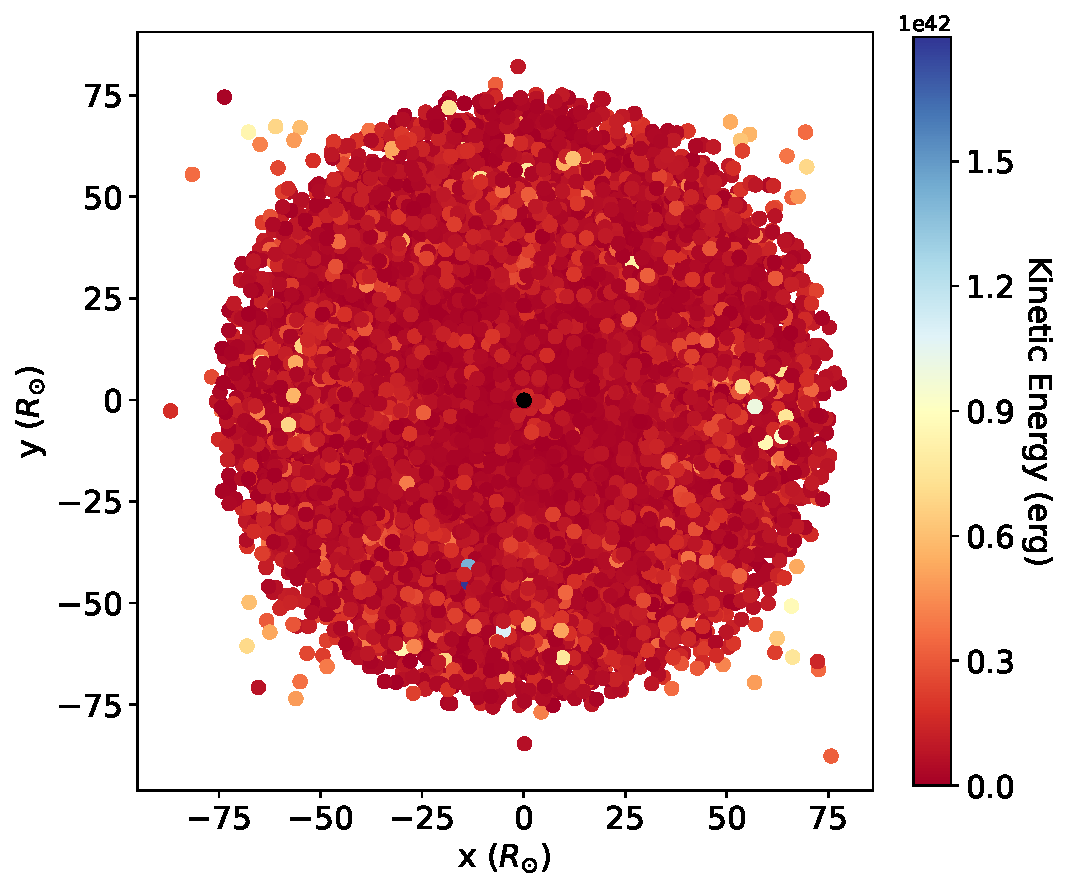
\includegraphics[width=\textwidth]{Thesis/graphs/tertiary_kin_energy_relaxed_2_5_tdyn.pdf}   
        \caption{Kinetic energies of the gas particles at  $t_{relax} = 2.5t_{dyn}$}%
    \end{subfigure}
    \hfill
    \begin{subfigure}[b]{0.49\textwidth}  
        \centering 
        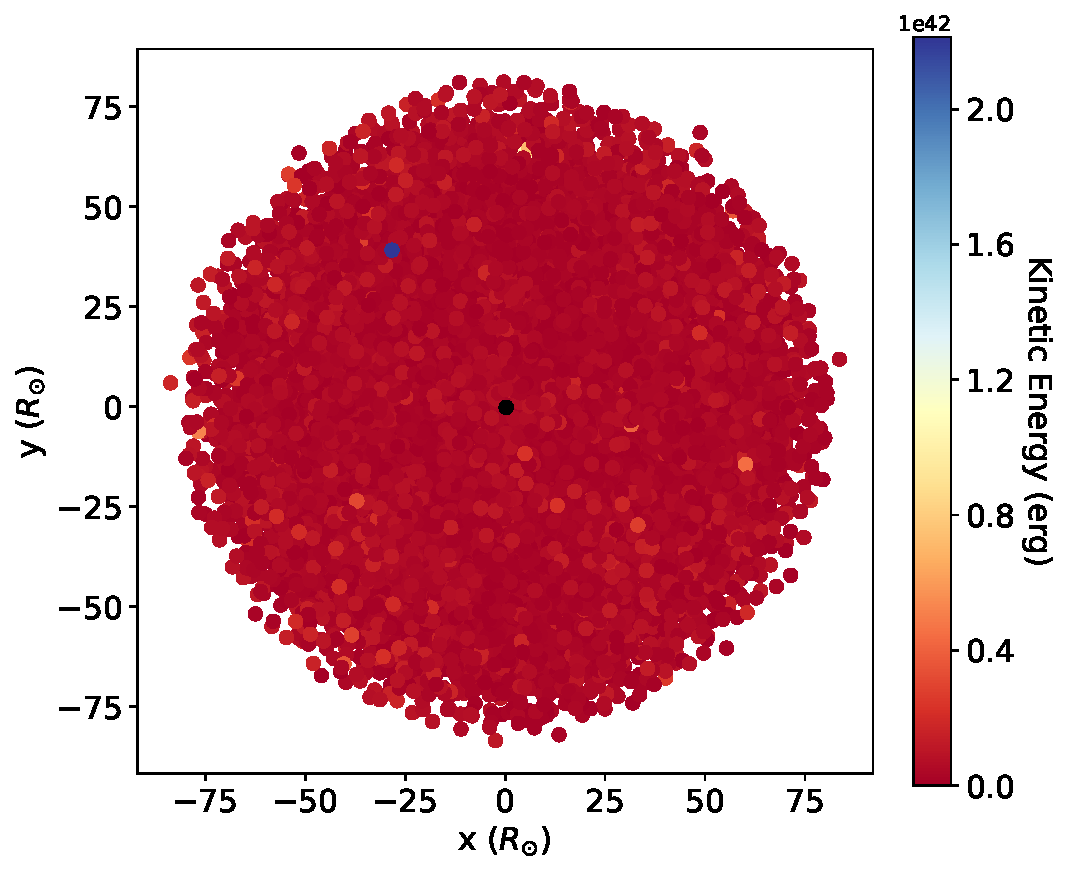
\includegraphics[width=\textwidth]{Thesis/graphs/tertiary_kin_energy_relaxed_5_tdyn.pdf}
        \caption[]%
        {{\small Kinetic energies of the gas particles at  $t_{relax} = 5t_{dyn}$}}
    \end{subfigure}
    \vskip\baselineskip
    \begin{subfigure}[b]{0.49\textwidth}  
        \centering 
        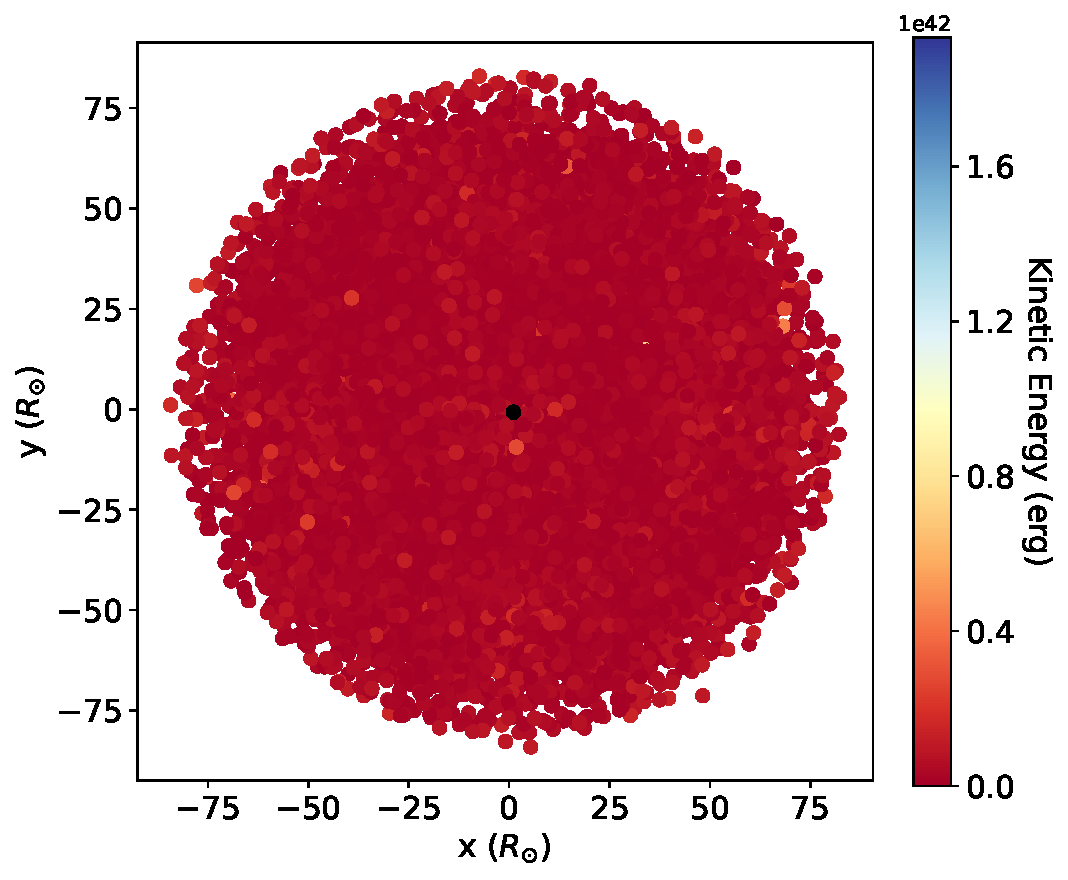
\includegraphics[width=\textwidth]{Thesis/graphs/tertiary_kin_energy_relaxed_7_5_tdyn.pdf}
        \caption[]%
        {{\small Kinetic energies of the gas particles at  $t_{relax} = 7.5t_{dyn}$}}
    \end{subfigure}
    \hfill
    \begin{subfigure}[b]{0.49\textwidth}  
        \centering 
        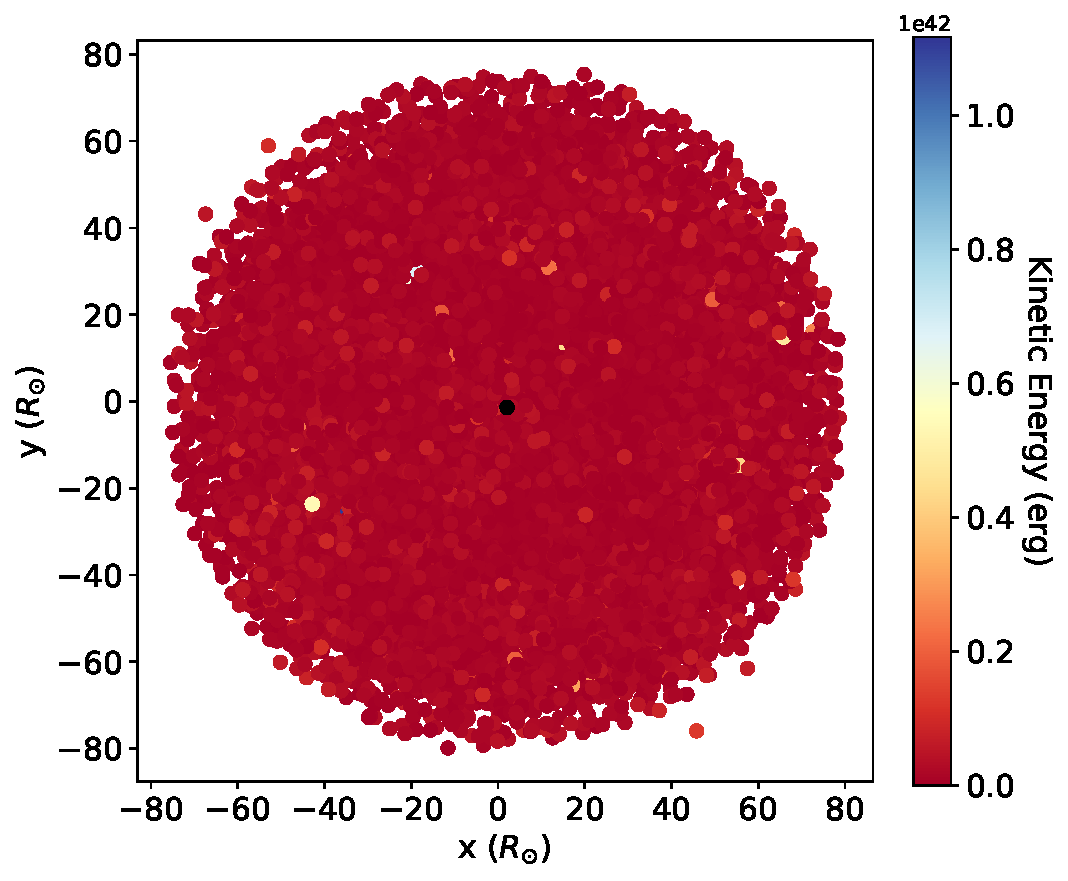
\includegraphics[width=\textwidth]{Thesis/graphs/tertiary_kin_energy_relaxed_10_tdyn.pdf}
        \caption[]%
        {{\small Kinetic energies of the gas particles at  $t_{relax} = 10t_{dyn}$}}
    \end{subfigure}
    \caption{2D maps of gas particles kinetic energies during relaxation.
    The chronological order is from left to right and from top to bottom as depicted on the respective labels. The black point corresponds to the core particle which is a pure gravitational point mass with no pressure or internal energy.}
    \label{fig:kin_energy_maps_relaxation}
\end{figure}
\cref{fig:kin_energy_maps_relaxation} shows the re-adjustment of particle positions and velocities based on \cref{eq:adjust_positions} and \cref{eq:adjust_velocities}. As the 3D hydrodynamical model becomes more spherically symmetric and the particles' kinetic energy decreases, it gradually moves towards a more hydrodynamically stable state. The latter is more apparent in \cref{fig:total_kin_energy_relaxation}, where
I present the total kinetic energy of the gas particles at $t_{relax} =[2.5, 5, 7.5, 10] t_{dyn}$.
\begin{figure}[H]
    \centering
    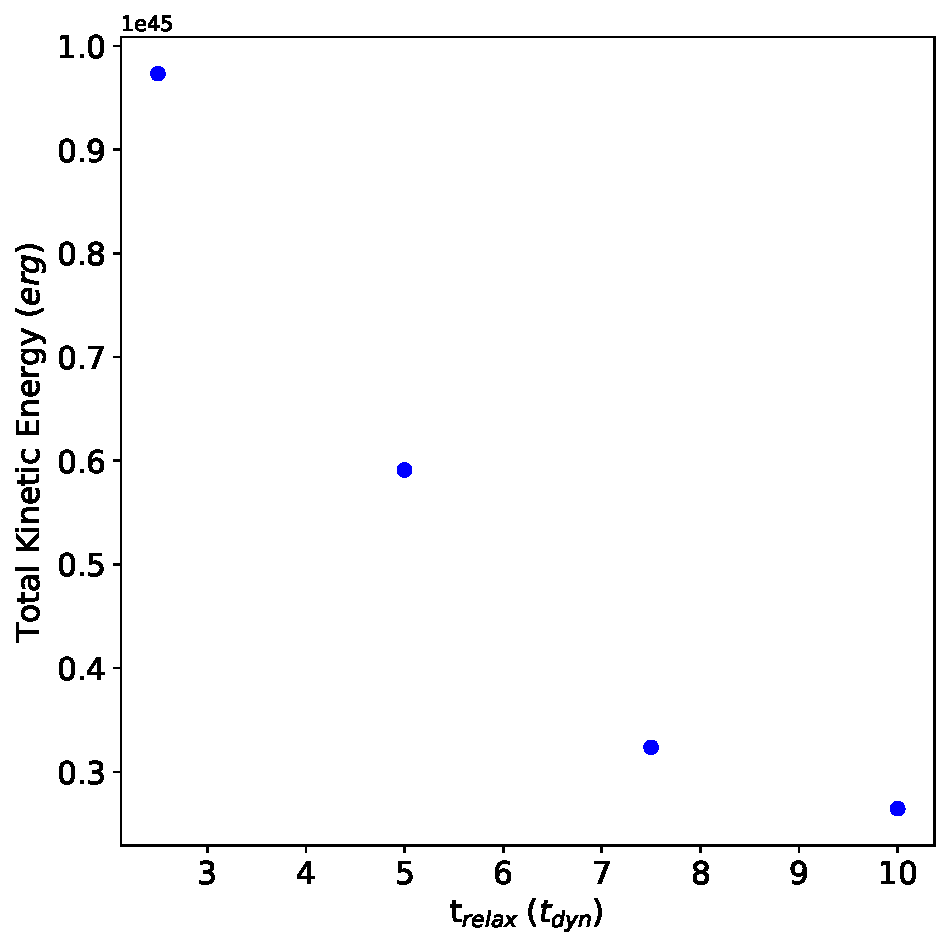
\includegraphics[width=0.9\textwidth]{Thesis/graphs/total_kientic_energy_during_relaxation.pdf}
    \caption{Evolution of the total kinetic energy of gas particles during relaxation. The blue points correspond to $t_{relax} =[2.5, 5, 7.5, 10] t_{dyn}$, respectively.}
    \label{fig:total_kin_energy_relaxation}
\end{figure}
















\section{Setting up the system}

The initial positions and velocities of the three stars are chosen such as they correspond to the orbital parameters given in \cref{tab:system_orbit_param}. The orientation of the inner orbit with respect to the outer orbit is defined by the inclination, $i$, longitude of the ascending note, $\Omega$, and argument of periastron, $\omega$ of the inner orbit relative to the outer orbit. Among these three parameters, mutual inclination is predicted to have the greatest influence on mass transfer, hence its a free parameter to be explored.  Additionally, I assume that  $\Omega=0^{\circ}$, effectively the line of nodes corresponds to the line connecting the inner binary components and $\omega= 90^{\circ}$. The effective potential of $\xi$ Tau corresponding to the initial configuration of the system is depicted in \cref{fig:triple_equop}.
\begin{figure}[H]
    \centering
    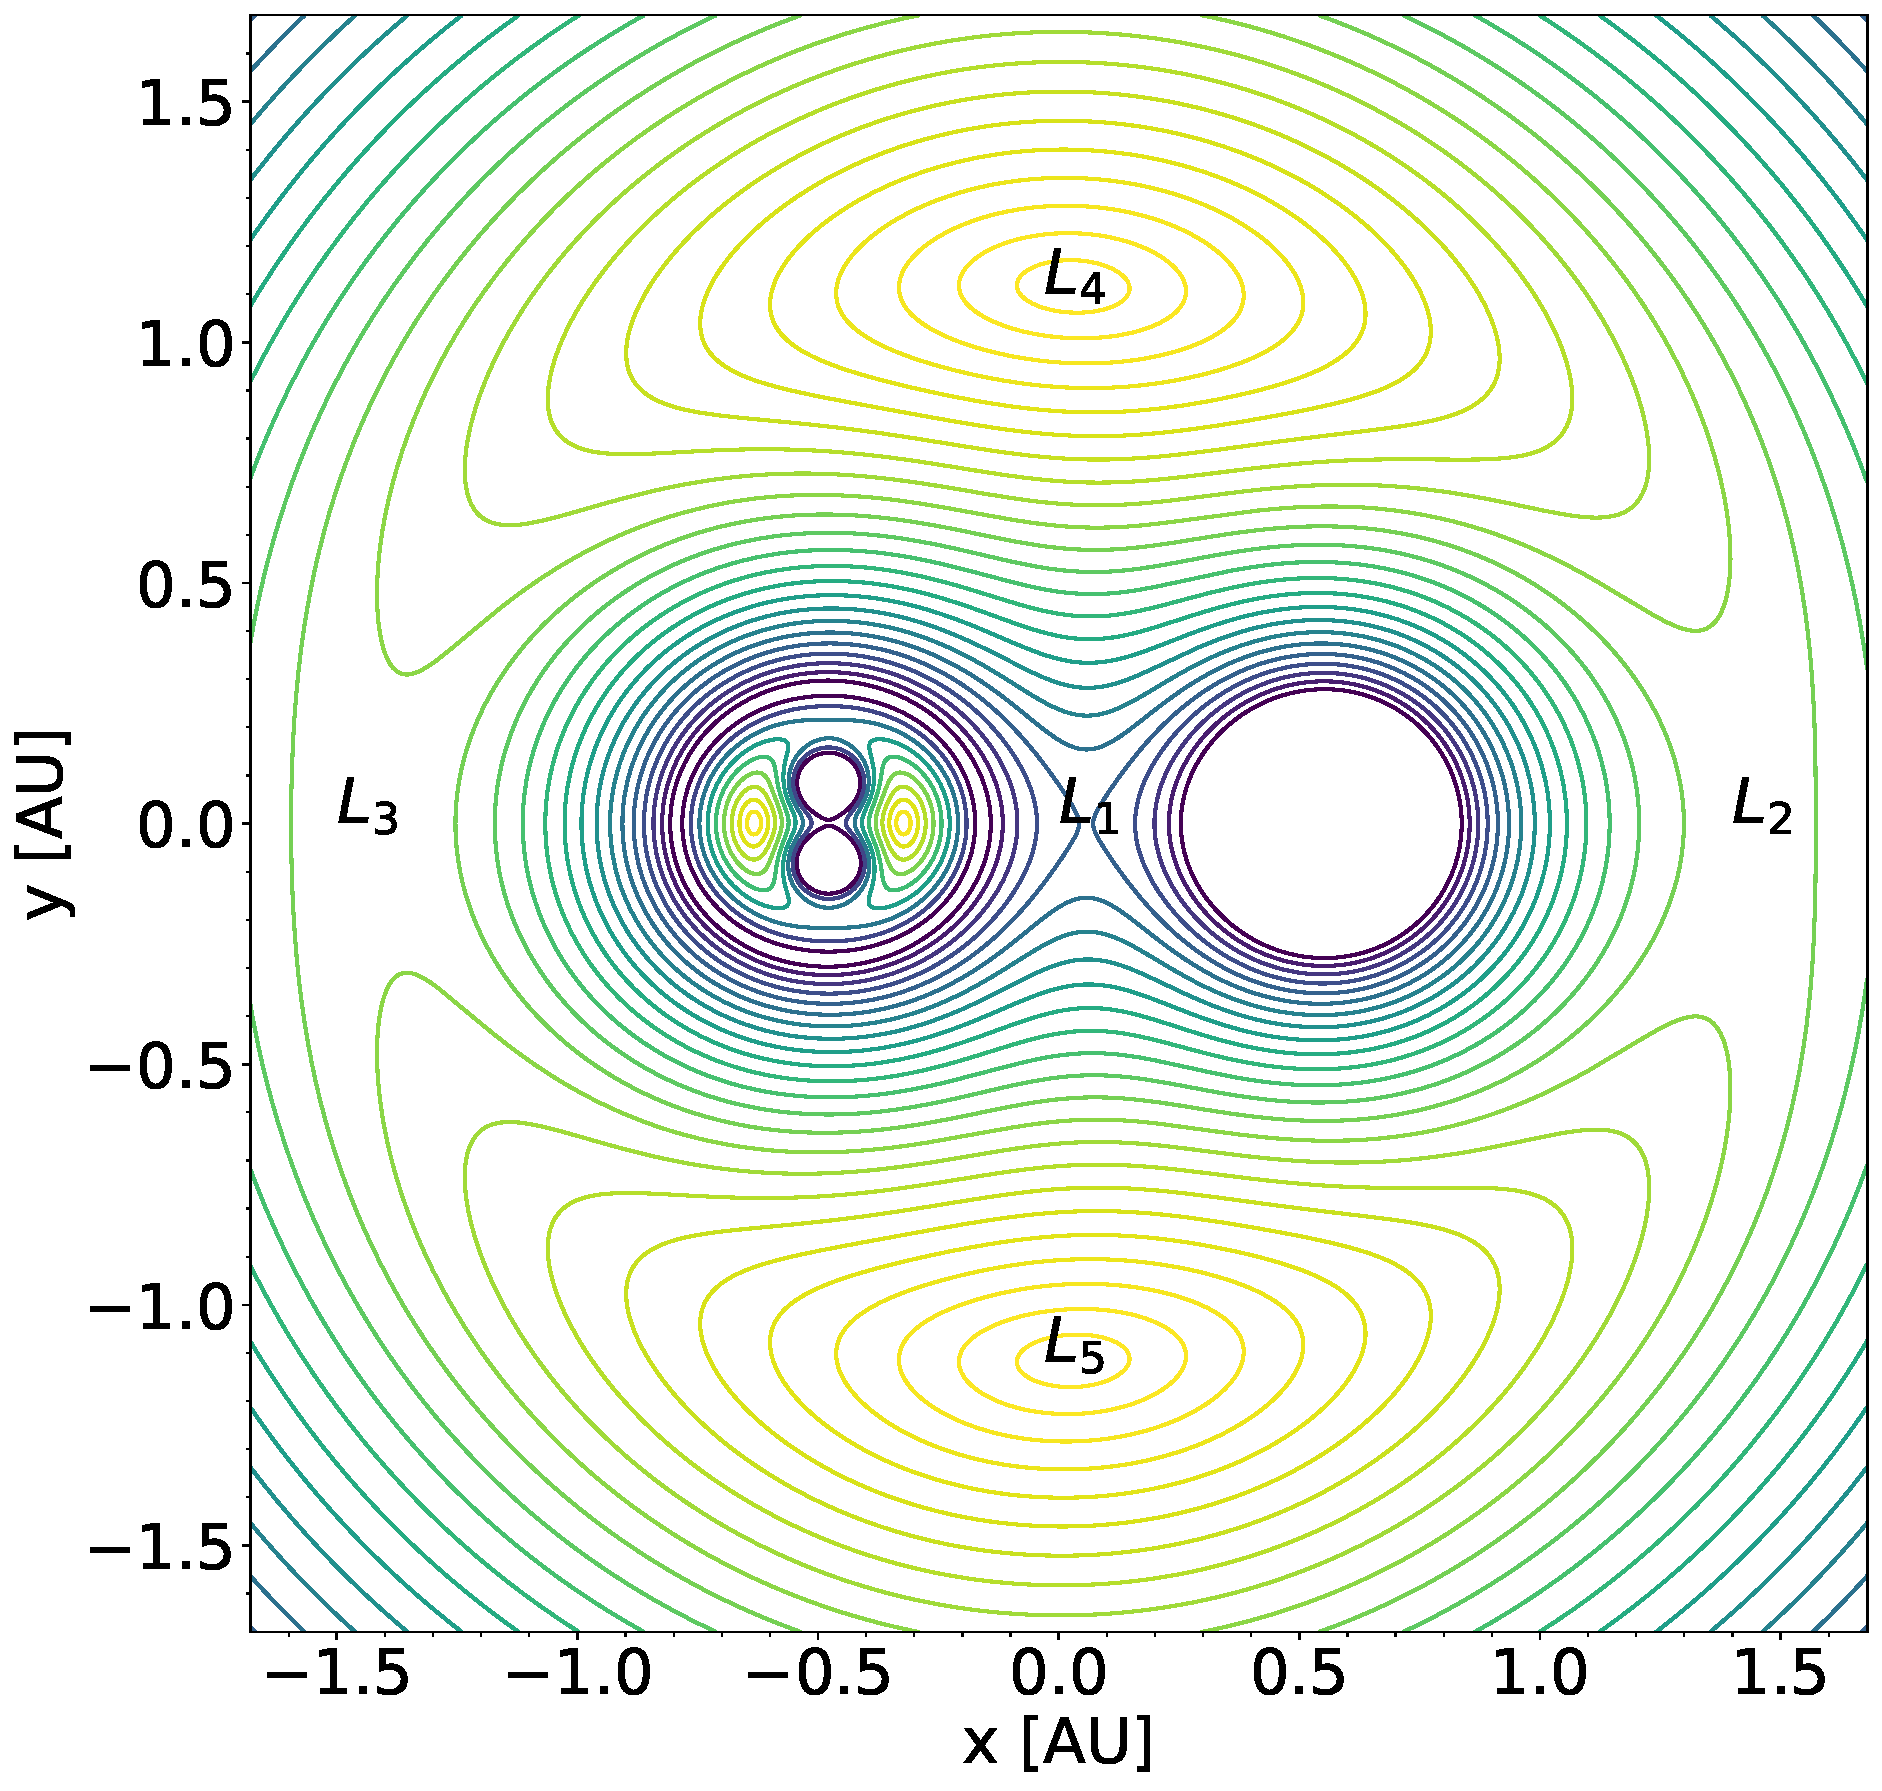
\includegraphics[width=0.9\textwidth]{Thesis/graphs/triple_equop.pdf}
    \caption{Contour plot of $\xi$ Tau's effective potential. The five Lagrangian points of the outer orbit are indicated as $L_1, L_2, L_3, L_4$ and $L_5$. I create this plot using the Hermite integrator which is part of  AMUSE \citep{hut1995building}.}
    \label{fig:triple_equop}
\end{figure}
After relaxing the 3D hydrodynamical model for $t_{relax} =10 t_{dyn}$, I have successfully created a fairly stable model, which represents the outer star. I now replace the outer star, which was a point mass until now, with the 3D hydrodynamical model. Based on the initial configuration the system is well inside the stable regime, see \cref{eq:stability_regime}, the octupole term, $\epsilon_{oct} = 0.00$, see \cref{eq:octupole_term}, thus it is not expected to be important, while the timescale of Lidov-Kozai cycles, see \cref{eq:lidov_kozai_timescale}, is $t_{koz}$ = 16.81 yr.
\section{Coupling hydrodynamics with gravity in the evolution model}

In order to encapture accurately all the details of system's evolution during mass transfer and in self consistent way, it is necessary to employ an accurate gravity solver and a method to handle the system's hydrodynamics. In general, SPH codes use low-accuracy gravity solvers and the details of the complex three-body gravitational dynamics may not be handled properly, e.g. the details of the Lidov-Kozai cycles. Hence, I employ the semi-symplectic direct N-body integrator Huayno, see \cref{sub:huayano}, to integrate equations of motion of the inner binary components, while the hydrodynamics and self-gravity of the 3D hydrodynamical model are handled by GADGET-2, see \cref{sub:gadget2}. 

In order to couple the two codes in the evolution model, I utilize the Astrophysical Multi-purpose Software Environment (AMUSE, \cite{pelupessy2013astrophysical,portegies2018astrophysical}), a comprehensive computational tool, to accurately simulate and solve for these physical processes in a self-consistent manner.  The software is written in Python and allows users to combine multiple astrophysical codes into a single simulation. 

\subsection{The bridge method}

The key feature of AMUSE is the Bridge method, first introduced by \cite{fujii2007bridge} and used to combine two different gravity solvers. The coupled integrator divides the Hamiltonian of the combined solution and iteratively integrates it with robust numerical integration techniques. As a result, the method can be implemented in general when the dynamics of a system can be divided into multiple regimes \citep{zwart2013multi}. In this section, I focus on coupling gravity and hydrodynamics which is the focus of this work.

\cite{saitoh2010fast} showed that the dynamical equations for SPH evolution can be derived from a Hamiltonian formalism, hence the Bridge formalism is applicable to a separation of purely gravitational and SPH particles. In my case, GADGET-2 (see \cref{sub:gadget2}) handles the self-gravity and hydrodynamics of the gas, while Huayano (see \cref{sub:huayano}) the gravitational dynamics of the inner binary. Using the Bridge method I achieve a second-order coupling between gravitational dynamics and hydrodynamics. As a result, the hydrodynamical solver is affected by the gravitational potential of its own particles as well as the gravitational potential of the inner binary. Furthermore, the hydrodynamics, namely gas drag, impacts the orbits of the two inner stars.
\begin{figure}[H]
    \centering
    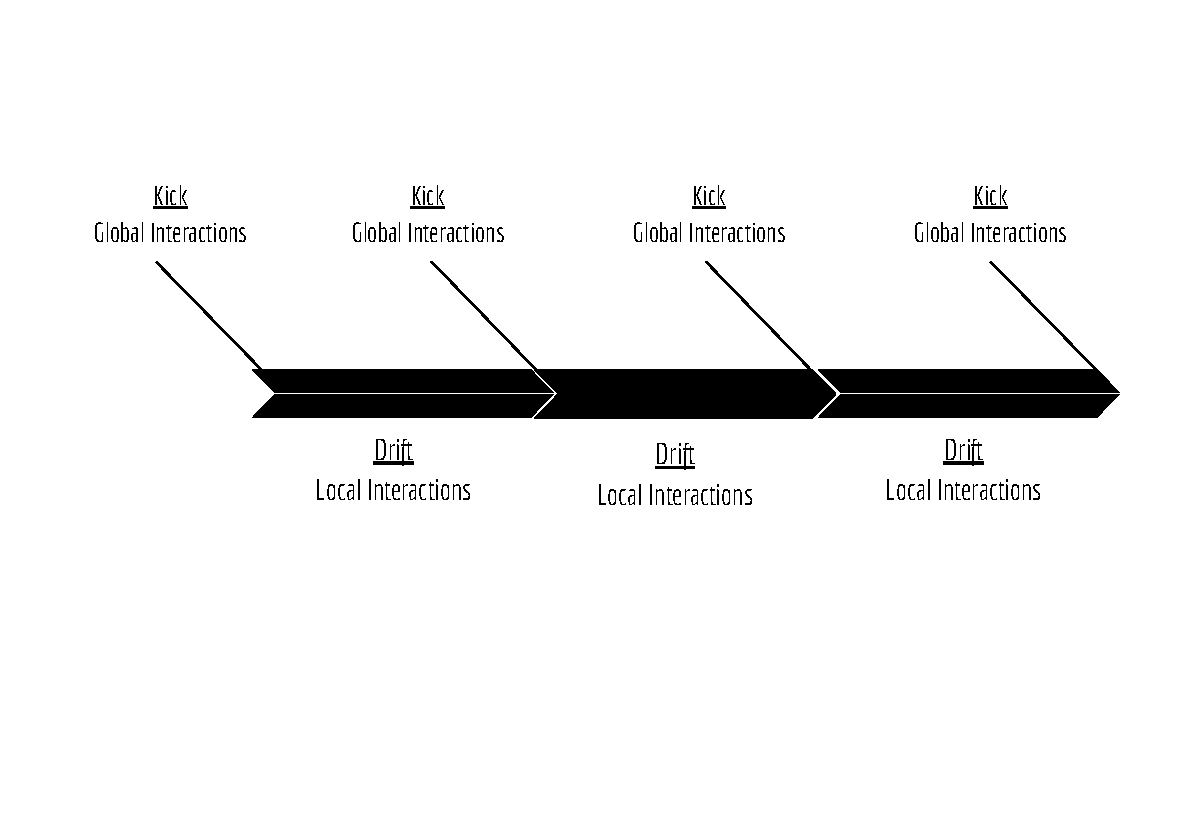
\includegraphics[width=0.9\textwidth]{Thesis/figures/kick_drift_kick.pdf}
    \caption{Schematic kick–drift–kick procedure.}
    \label{fig:kick_drift_kick}
\end{figure}
The evolution via the Bridge method can be implemented as a kick–drift–kick scheme, as illustrated in \cref{fig:kick_drift_kick}. More specifically:
\begin{enumerate}
    \item Kick (Inner Binary, Huayano): Initially, Huayano is used to calculate the gravitational forces operating on the inner binary. These forces "kick" the point masses, causing them to change velocity.
    \item Drift (Inner Binary, Huayano): With the revised velocities of the point masses, Huayano is used to evolve their positions forward in time, assuming a constant velocity over a short time period.
    \item Kick (Tertiary, GADGET-2): At this point, Bridge is used to transmit the modified positions and velocities of the point masses from Huayano to GADGET-2. The latter utilizes these positions to determine the gravitational forces exerted by the point masses on the 3D hydrodynamical model. These forces "kick" the SPH particles and the core particle, causing their velocities to change.
    \item Drift (Tertiary, GADGET-2): Now, using the updated velocities of the 3D hydrodynamical model, GADGET-2 evolves the particles positions forward in time allowing for fluid flow and interactions based on the combined effects of gravity and hydrodynamics.
    \item Kick (again) (Inner Binary, Huayano): Once again, Bridge is used, to transport the new positions and velocities of the 3D hydrodynamical model from GADGET-2 back to Huayano. Huayano recalculates the gravitational forces acting on the point masses by the 3D hydrodynamical model. These forces "kick" the point masses once more, causing their velocities to change.
    \item Drift (again) (Inner Binary, Huayano): Finally, with the updated velocities of the point masses, Huayano is used to evolve their positions forward in time again, assuming a constant velocity over a short time period.
\end{enumerate}

Each code operates on their own internal time steps, while the Bridge time step defines the time interval at which the codes interact with each other. Hence, its an important parameter to accurately model the coupling between hydrodynamics and gravity. Nevertheless, a time step, $t_{bridge}$, which is about a fraction of $1/64$ the inner binary orbital period, see \cref{tab:system_orbit_param}, provides converged solutions. 




\section{Codes' set up}

At this point, it is clear that I took many consecutive steps to model mass transfer in triple systems with a Roche-lobe filling outer star. A schematic representation of the entire process is provided in \cref{fig:schematic_method}
\begin{figure}[H]
    \centering
    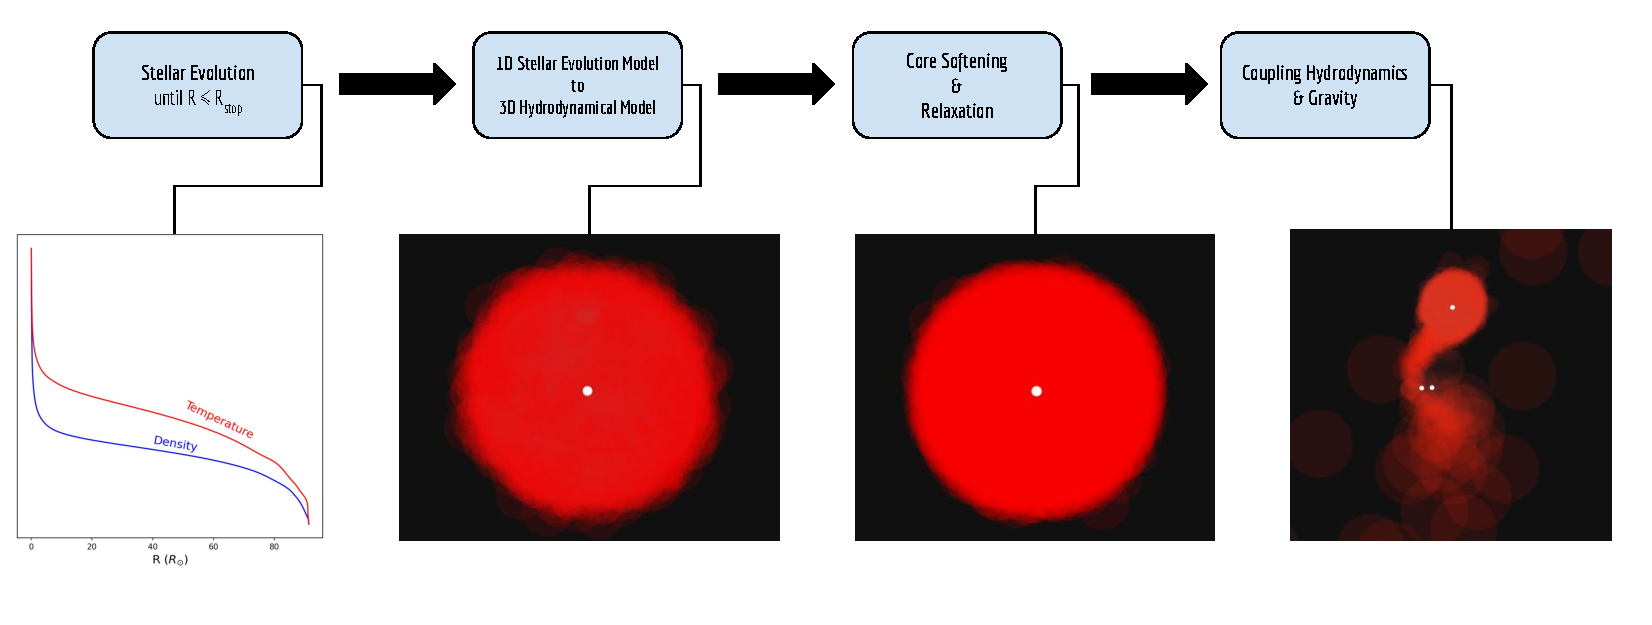
\includegraphics[width=\textwidth]{Thesis/figures/method_schematic.pdf}
    \caption{Schematic representation of the steps taken to simulate mass transfer in the triple system with a Roche-lobe filling outer star. The white points are the purely gravitational particles representing the core and the inner binary components. The red points are the \ac{sph} particles representing the gas having an adaptive smoothing length.}
    \label{fig:schematic_method}
\end{figure}
In each step, I explored the importance of different parameters and made assumptions based on relative physics to better simulate the system's behavior. The outcome of a simulation is, of course, dependent on the simulation's setup; Furthermore, knowing the setup parameters is important for the reproducibility of the results. Hence, I summarize the codes' settings used for the final simulations for the reader.
\begin{table}[H]
    \centering
    \begin{tabular}{ |p{6.5cm}||p{6.5cm}|  }
     \hline
     \multicolumn{2}{|c|}{Code Settings} \\
     \hline
     MESA & GADGET-2 \\
     \hline
     Initial Masses = [3.2, 3.1. 5.5] M$_{\odot}$& $N_{particles}=50^4$ \\
     Solar metallicity& Self-gravity: True\\
     No winds& Adaptive smoothing length: True\\
     No overshooting& Softening = smoothing length\\
     No star rotation & Adiabatic \ac{eos}  \\
     Convection-occurrence (Schwarzwild) & Time step = $1/64 \times P_{in}$ \\
     Evolve until $\geq 1.1 \times R_{RLOF}$ & Artificial viscosity: $\alpha=0.5, \beta=1.0, \eta=0.1$ \\
     \hline
    \end{tabular}
        \centering
    \begin{tabular}{ |p{6.5cm}||p{6.5cm}|  }
     \hline
     \multicolumn{2}{|c|}{Code Settings} \\
     \hline
     Huayno & AMUSE \\
     \hline
     No softening length & Gravity-Hydrodynamics (2nd-order-coupling)\\
     Default time step ($<< 1/64 \times P_{in}$) &  Bridge time step = $1/64 \times P_{in}$\\
     \hline
    \end{tabular}
    \caption{ Various important settings and flags used for the different codes and AMUSE}
\label{tab:codes_settings}
\end{table}
